\section{Theory}
\label{sec:theory}
Since we want to highlight the historical importance of the discovery of the Compton effect, we introduce the theoretical 
backgrounds in close relation to the questions asked at the beginning of the last century. Taking this perspective, we 
review the theories existing prior to Compton's explanation and their points of failure. His "new" quantum mechanical 
approach yielded two central results: the prediction of a shift in wavelength and a cross section dependent on the 
wavelength of the incident radiation. Both features are described on the following pages. 

\subsection{Failure of Thomson scattering}
\label{sec:thomson}
At the beginning of the 1920s, the nature of electromagnetic radiation was still subject of a large debate within the 
physics community. Although Einstein had shown the particle-like character of light in case of the photoelectric effect, 
this picture was nowhere near being widely accepted. Instead, most theories based on classical electrodynamics and people 
were using quite complicated deviations in order to stay with the classic theory. Reading Compton's original paper, one is 
confronted with a vivid description of these seemingly desperate attempts.\cite{compton} 
To understand these difficulties, we introduce the 
theory of Thomson scattering, a classical description of elastic scattering of electromagnetic radiation at charged 
particles. In our case, we deal with electrons. These are accelerated by the electric field and will thus act as Hertzian 
dipoles. They emit radiation of the same frequency as the incident rays, in terms of wavelength:
\begin{equation}
    \lambda_\text{Th}' - \lambda = 0\, ,	
    \label{eq:thomsom_lamb}
\end{equation}
where $\lambda$ denotes the wavelength of the incident radiation and $\lambda_\text{Th}'$ the one of the scatter rays.
For radiation of low frequency (soft X-rays and lower), this had been successfully tested experimentally. However, for 
hard X-rays and $\gamma$-rays, the observations were contradictory: The wavelength of scattered light was higher. Compton 
previously tried to ascribe this to fluorescence, but after conducting his experiment, he found it "difficult to attribute
it to anything other then true scattering"\cite{compton}. 

The second substantial disagreement between the acquired experimental data and Thomson's theory was the cross section of 
the scattering in the regime of hard X-rays and $\gamma$-rays. The classical theory yields a cross section independent of 
the wavelength of incident radiation. The differential cross section dependent on the scattering angle $\theta$ is given by
\begin{equation}
    \begin{split}
        \frac{\text{d} \sigma_\text{Th}}{\text{d} \Omega} 
        &= \frac{1}{2} \left(\frac{e^2}{m_e c^2}\right)^2 \left(1 + \cos^2 \theta  \right)  \\
        &= \frac{1}{2} r_e^2 \left(1 + \cos^2 \theta  \right) 
        \label{eq:thomson}
    \end{split}
\end{equation}
with the classical electron radius $r_e = e^2/m_e c^2$. 
The total cross section is then calculated by integrating over the entire sphere:
\begin{equation}
    \begin{split}
        \sigma_\text{Th, total} &= \int_\Omega \! \frac{\text{d} \sigma_\text{Th}}{\text{d} \Omega}  \, \text{d}\Omega \\
            &= \left(\frac{1}{2} r_e^2\right)  2\pi \int_0^\pi \! \left(1 + \cos^2\theta\right)\sin\theta \, \text{d}\theta \\
            &= r_e^2\pi \left[ -\cos\theta -\frac{1}{3}\cos^3\theta \right]_0^\pi \\
            &= \frac{8\pi}{3} r_e^2 
        \label{eq:total_thomson}
    \end{split}
\end{equation}
Inserting the numerical values, we get a cross section of $\sigma_\text{Th, total} = 66.524 \text{ fm}^2$. 
However, in the regime in question the cross section turned out to be considerably lower. An idea put forward prior to 
1923 was the "large electron", having a radius comparable to that of the wavelength of X-rays or $\gamma$-rays. Compton's
experiment wrecked these attempts because it turned out that the radius would have to adapt to the wavelength of the 
radiation.\cite{compton}   

A third difficulty of the classical theory was the description of the discrete nature of scattering events in the case of 
low intensity incident radiation. Today, this is of course interpreted from the perspective of photons being discrete 
quanta of light. In the classical theory, however, one assumed a continuous electrical field acting on the entire sample
with the scattered radiation as a result of interference. 

Notwithstanding all these problems, Thomson's theory remains an important tool e.~g. in plasma physics, as it turns out to
be the limit of th quantum mechanical description in the regime of low energy, essentially for incident frequencies 
$\nu \ll \frac{m_ec^2}{h}$. At this point, nonetheless, we will turn back to our central subject which overcame all of the
stated problems and had a large influence on the following change in paradigm. 

\subsection{Shift in wavelength}
\label{sec:wavelength}
\begin{figure}[htpb]
    \centering
    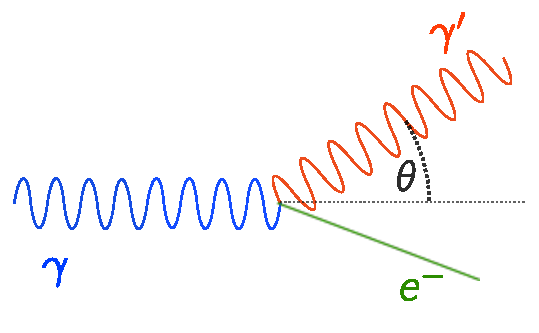
\includegraphics[width=0.8\linewidth]{figures/compton_scatter}
    \caption{
        Scheme of Compton scattering in the rest frame of the electron prior to the scattering event. The photon before and
        after the scattering are distinguished by $\gamma$ and $\gamma'$ respectively. 
        }
    \label{fig:compton_scatter}
\end{figure}
Compton's picture in order to explain the observed phenomena was that of a elastic scattering between a quasi-free electron
and an incident photon. A sketch of this situation in the rest frame of the electron is shown in 
figure~\ref{fig:compton_scatter}. With this picture, the assumption of the conservation of energy \textit{and} momentum 
becomes natural. In the following, we use this axiomatic approach to derive and expression for the difference in
wavelength $\lambda' - \lambda$ at angle $\theta$. Energy conservation reads 
\begin{equation}
    E_\gamma + E_e =  E_{\gamma'} + E_{e'} \, .
    \label{eq:energy_conservation}
\end{equation}
When inserting an expression for the electron energy ($E_e = c\sqrt{p_e^2 + m_e^2c^2}$ with momentum $p_e$), this becomes 
\begin{align}
    E_\gamma + m_ec^2 &= E_\gamma' + \sqrt{p_{e'} + m_e^2c^2} \\
    \Rightarrow \qquad p_{e'}^2c^2 &= \left(E_\gamma - E_\gamma' + m_ec^2\right)^2 - m_e^2c^4 \, .
    \label{eq:energy2}
\end{align}
The momentum conservation 
\begin{equation}
    p_\gamma = p_{\gamma'} + p_{e'}	
    \label{eq:momentum_conservation}
\end{equation}
with $p_\gamma = E_\gamma/c$ yields
\begin{equation}
    \begin{split}
        p_{e'}^2c^2  &= \left(p_\gamma - p_{\gamma'}\right)^2c^2 \\
                     &= E_\gamma^2 +  E_\gamma'^2 - 2E_\gamma E_\gamma'\cos\theta \, .
        \label{eq:mom2}
    \end{split}
\end{equation}
Combining equations \eqref{eq:energy2} and \eqref{eq:mom2}, we get
\begin{align}
    &(E_\gamma - E_\gamma' + m_ec^2)^2 - m_e^2c^4 	&=& E_\gamma^2 +  E_\gamma'^2 - 2E_\gamma E_\gamma'\cos\theta \\
    \Rightarrow \qquad &-2E_\gamma E_\gamma' + 2(E_\gamma - E_\gamma')m_ec^2 &=& -2E_\gamma E_\gamma'\cos\theta \\
    \Rightarrow \qquad &(E_\gamma - E_\gamma')m_ec^2 &=& -E_\gamma E_\gamma'(1 - \cos\theta) \, .
    \label{eq:en_mom}
\end{align}
When dividing by $E_\gamma E_\gamma'$, we get a relation for the difference in wavelength 
\begin{equation}
    \lambda' - \lambda = \lambda_C(1 - \cos\theta)	
    \label{eq:compton1}
\end{equation}
where $\lambda = \frac{c}{\nu} = \frac{h c}{E_\gamma}$ and 
\begin{equation}
    \lambda_C = \frac{h}{m_ec} = 2.426 \text{ fm} 
    \label{eq:compton_wavelength}
\end{equation}
is called the "Compton wavelength". 
Introducing the reduced incident energy 
\begin{equation}
    a := \frac{E_\gamma}{m_ec^2}    \label{eq:ered}
\end{equation}
of the incident photon, the ratio of outgoing and incident photon frequency is conveniently written as 
\begin{equation}
    \frac{E_\gamma'}{E_\gamma} = \frac{1}{1 + a(\cos\theta)}	\, ,
    \label{eq:freq_rati}
\end{equation}
representing an ellipse with an eccentricity increasing with $a$.\cite{siegbahn2012alpha} 
The limit $a \ll 1$ corresponds to Thomson scattering: $\nu' = \nu$. 
We can further state the kinetic energy of the Compton recoil electron in the non-relativistic approximation. A 
straightforward calculation yields\cite{siegbahn2012alpha} 
\begin{equation}
    \begin{split}
        E_{e, \text{kin}} &= E_\gamma - E_\gamma' \\
                     &=  E_\gamma \frac{a (1 - \cos\theta)}{1 + a(1 - \cos\theta)} \, .
        \label{eq:ekin}
    \end{split}
\end{equation}
Both this kinetic energy and the energy of the photon are accessible experimentally with the setup we are using. 
In order to get an intuition of what is to be expected, we plot both energies in figure~\ref{fig:theory_conservation}.

\begin{figure}[htpb]
    \centering
    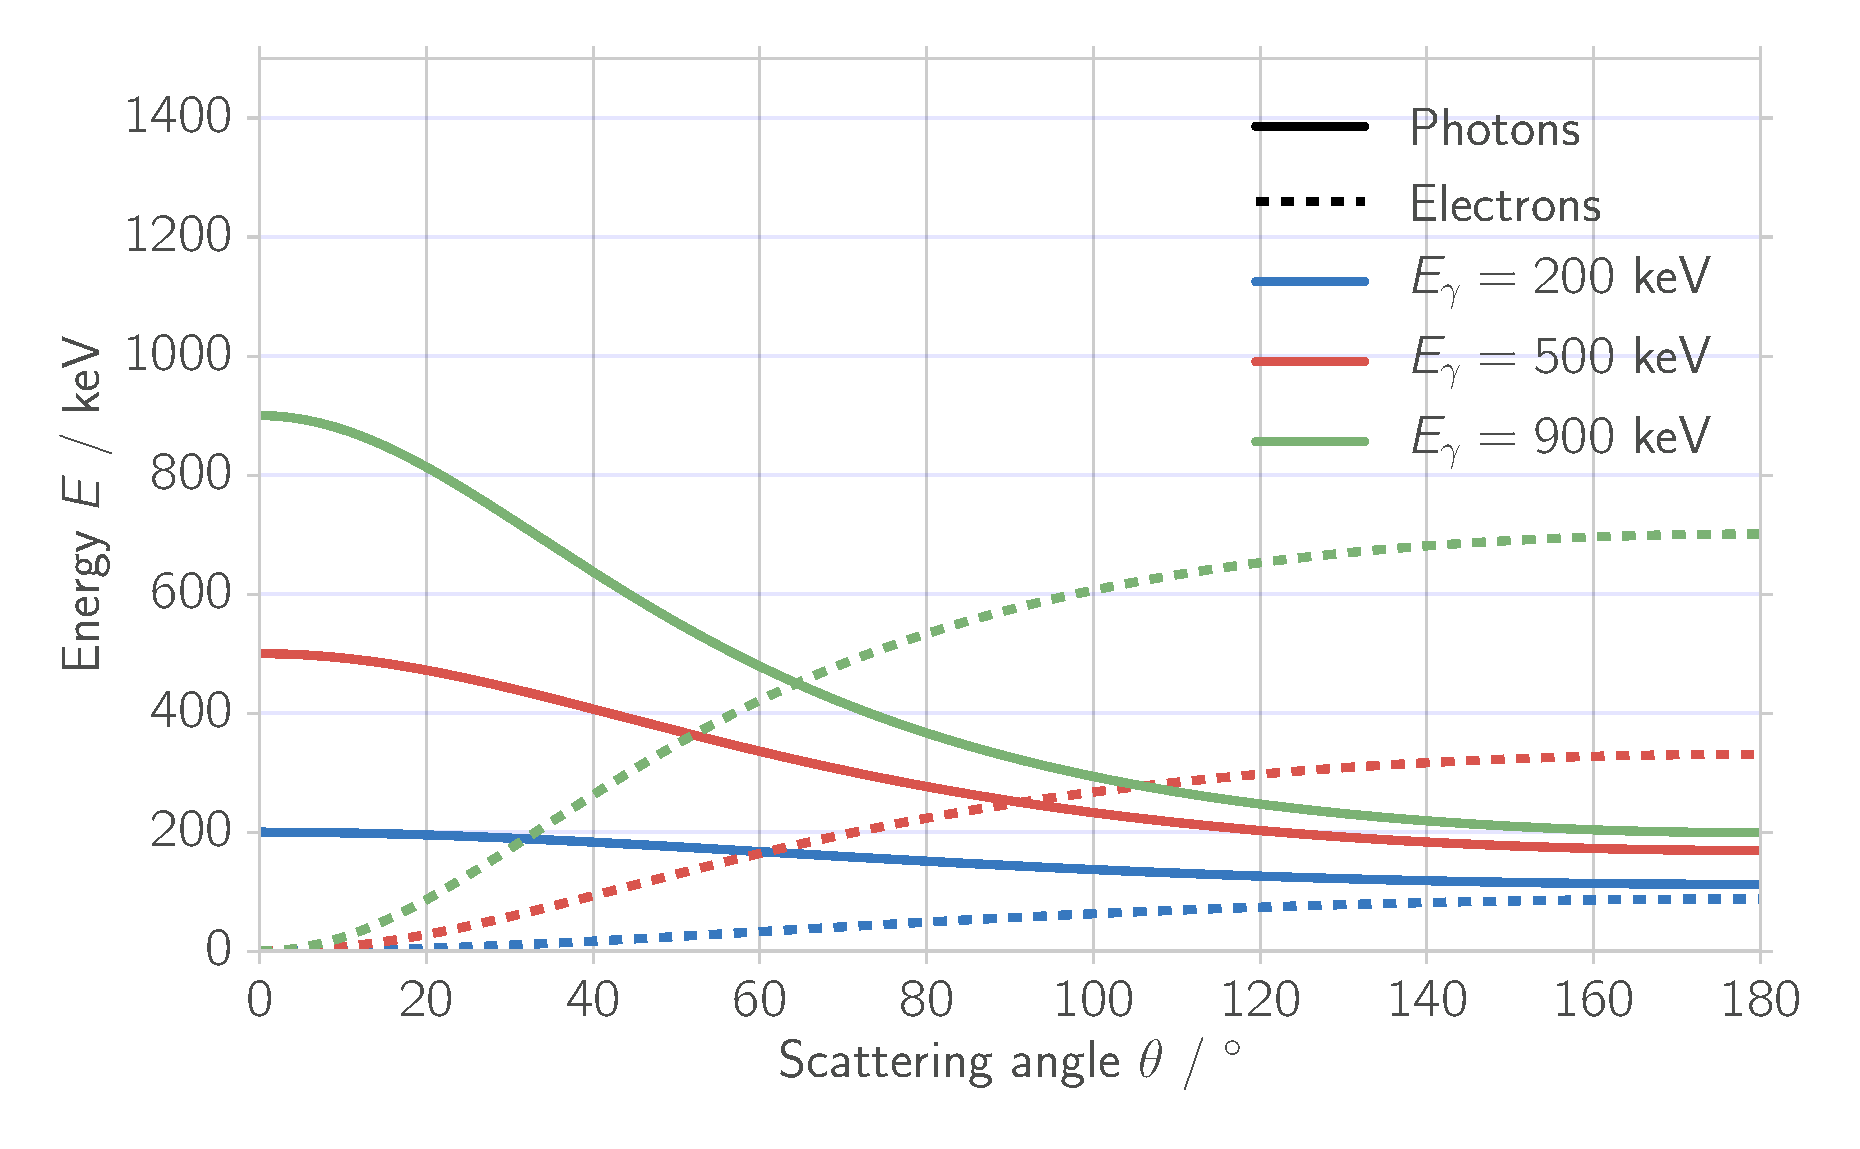
\includegraphics[width=0.8\linewidth]{analysis/figures/theory_conservation}
    \caption{
        Calculated energies of scattered photon and electron over the scattering angle of the photon for three different
        energies $E_\gamma$ of incident photons.
        The continuous line corresponds to the energy of the scattered photon, the dashed to the kinetic energy of the
        electron. The total energy is equal to $E_\gamma$ and (by definition) conserved in this non-relativistic 
        approximation. 
        }
    \label{fig:theory_conservation}
\end{figure}

From the expressions above, we can also deduce the maximal energy of the electron, which corresponds to the case of 
backscattering, i.~e. $\theta = 180^\circ$. Inserting $\cos \pi = -1$ into equation \eqref{eq:ekin} yields the
\textit{Compton edge} $ E_C$ to an according photo peak: 
\begin{equation}
    E_C = \frac{E_\gamma}{1 + \frac{1}{2a}}	
    \label{eq:e_max}
\end{equation}

\subsection{Cross section}
\label{sec:cross_section}
The derivation of the cross section for Compton scattering was one of the first results obtained with quantum 
electrodynamics. This was obtained in 1928 by Oskar Klein and Yoshio Nishina. This Klein-Nishina formula is the lowest 
order contribution of photons scattered by a single free electron. We will not restate its derivation 
but only give the final result for unpolarized light. The differential cross section in this case 
is\cite{schmueser2011feynman}
\begin{equation}
    \begin{split}
        \frac{\text{d} \sigma_\text{C}}{\text{d} \Omega} 
        &= \frac{\alpha^2 \lambda_e^2}{8 \pi^2} \frac{1}{\rho^2}\left(\rho + \frac{1}{\rho} - \sin^2\theta\right) ,
        \label{eq:kn_diff}
    \end{split}
\end{equation}
with 
\begin{equation}
    \rho := \frac{E_\gamma}{E_{\gamma'}}  = 1 + a(1 - \cos\theta) 
    \label{eq:rho}
\end{equation}
and the fine structure constant $\alpha = \frac{1}{4 \pi \varepsilon_0} \frac{e^2}{\hbar c}$.   
It is plotted for three different incident photon energies $E_\gamma$ in figure~\ref{fig:theory_diff_cs}. 

We calculate the total cross section as before:\cite{ver}
\begin{equation}
    \begin{split}
        \sigma_\text{C, total} &= \int_\Omega \! \frac{\text{d} \sigma_\text{C}}{\text{d} \Omega}  \, \text{d}\Omega \\
            &= \frac{\alpha^2 \lambda_e^2}{8\pi^2} \int_0^{2\pi} \! \int_0^{\pi} \! 
        \frac{1}{\rho^2}\left(\rho + \frac{1}{\rho} - \sin^2\theta\right) \sin\theta \, \text{d}\theta  \, \text{d}\phi \\
        &=\frac{\alpha^2 \lambda_e^2}{2\pi a^2} \left(
            \frac{2 + a(1 + a)(8 + a)}{(1 + 2a)^2} + 
            \frac{(a - 1)^2 - 3}{2a} \cdot \ln(1 + 2a)\right)   \,.
        \label{eq:total_compton}
    \end{split}
\end{equation}
A plot of the total cross section can be observed in figure~\ref{fig:theory_total_cs}. In order to interpret our 
experimental data, we need to perform a transformation of variables to the kinetic energy of the electron. This 
yields\cite{ver}
\begin{equation}
    \frac{\text{d} \sigma_\text{C}}{\text{d} \Omega} 
    = \frac{\alpha^2 \lambda_e^2}{16 \pi^3 m_e c^2}  \frac{1}{a^2}\left(
        \frac{b^2}{a^2(a - b)^2} + \frac{(b - 1)^2 - 1}{a (a - b)} \right) ,
    \label{eq:dode}
\end{equation}
with reduced electron energy $b := E_{e, \text{kin}} / m_ec^2$. This differential cross section is shown in 
figure~\ref{fig:theory_dsde}.

\newcommand{\picwidth}{0.48\textwidth}
\begin{figure}
    \begin{subfigure}[b]{\picwidth}
        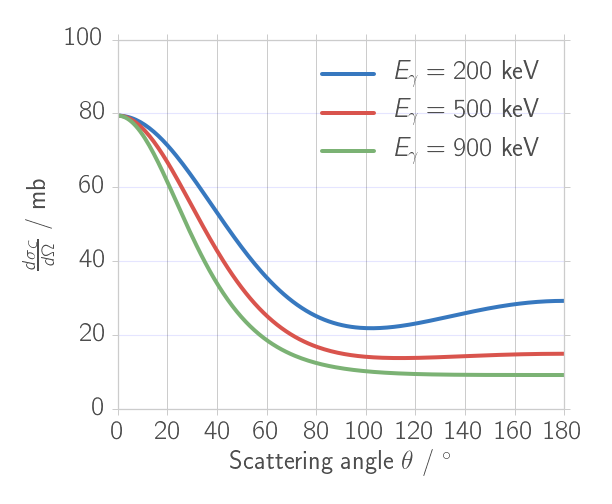
\includegraphics[width=\linewidth]{analysis/figures/theory_diff_cs}
        \subcaption{$\,$}
        \label{fig:theory_diff_cs}
    \end{subfigure}\quad
    \begin{subfigure}[b]{\picwidth}
        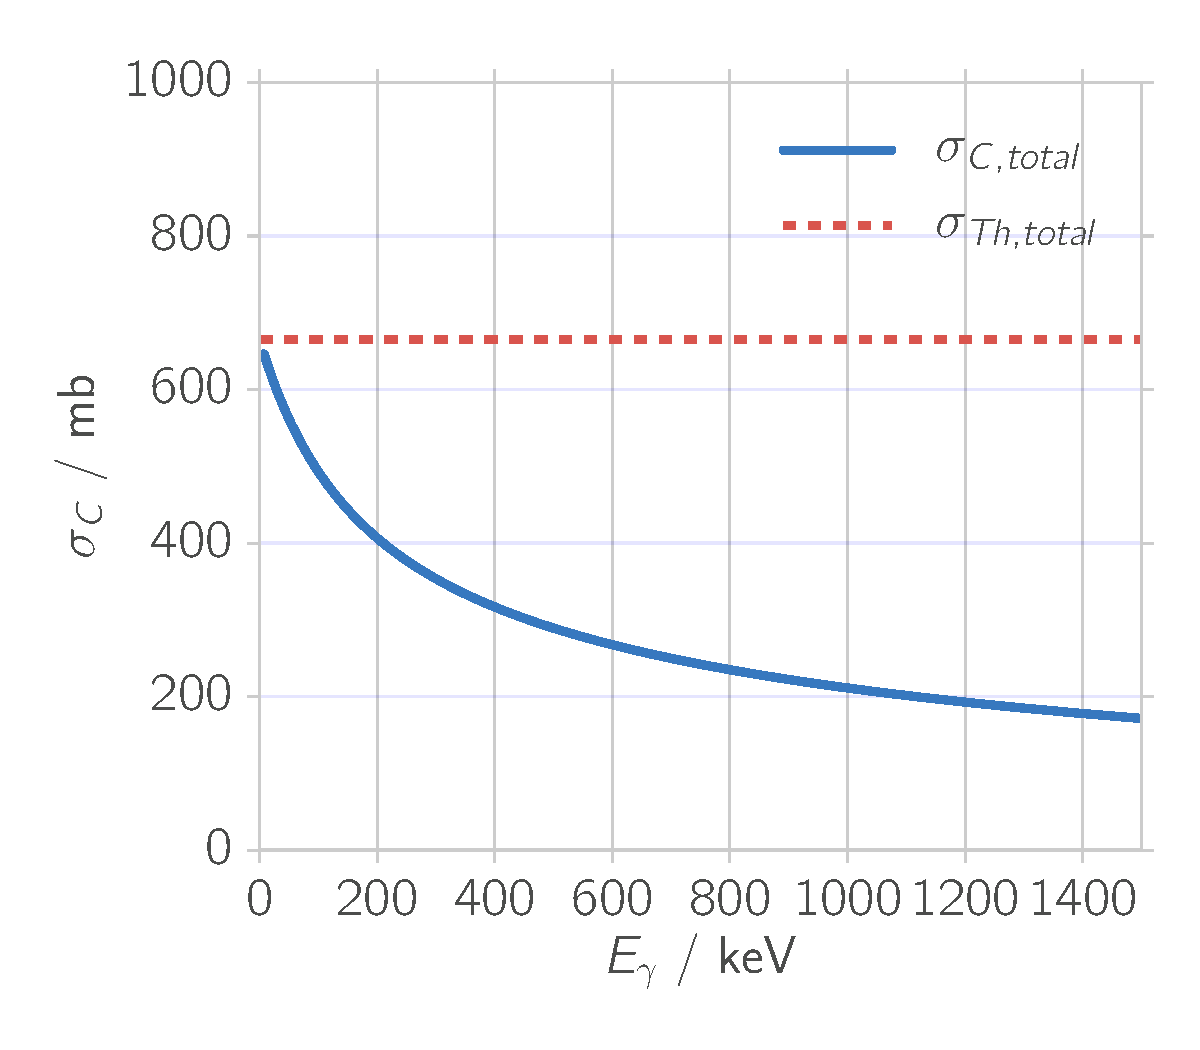
\includegraphics[width=\linewidth]{analysis/figures/theory_total_cs}
        \subcaption{$\,$}
        \label{fig:theory_total_cs}
    \end{subfigure}
    \caption{Cross sections for Compton scattering as derived by Klein and Nishina. (\subref{fig:theory_diff_cs}): 
        Differential cross section i.~e. the Klein-Nishina formula over the scattering angle of the photon 
        for three different incident photon energies. In our experiment, the photon energy of the Cs-sample is 
        $E_{\gamma, \text{Cs}} = 662$ keV. (\subref{fig:theory_total_cs}): Total cross section over incident photon 
        energy for Compton and Thomson scattering.
    }
    \label{fig:theory_cross_section}
\end{figure}

\begin{figure}[htpb]
    \centering
    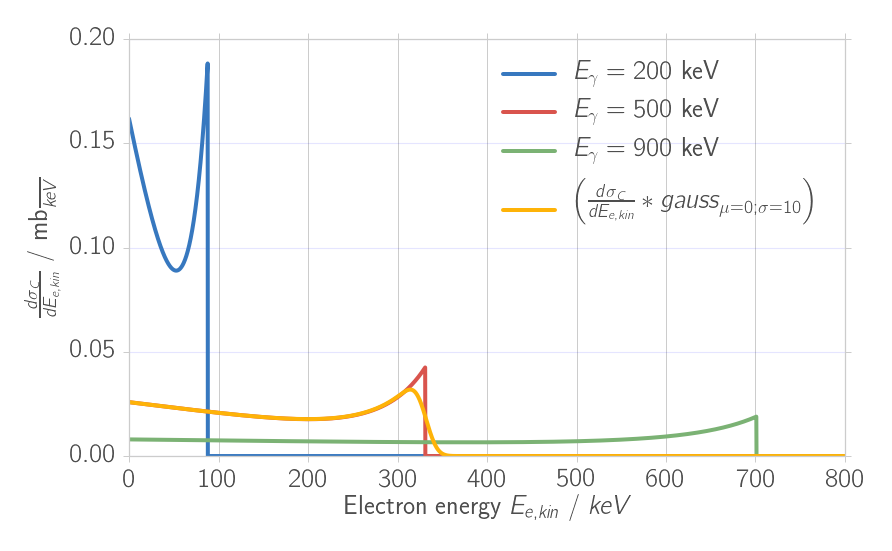
\includegraphics[width=0.8\linewidth]{analysis/figures/theory_dsde}
    \caption{
        Differential cross section in terms of electron energy $E_{e, \\text{kin}}$. The discontinuous edges 
        are the respective Compton edges $E_C$. Experimental results are expected to be smeared, i.~e. convoluted with a 
        normal distribution. The yellow line is such a convolution, here with the differential cross section at
        $E_\gamma = 500$ keV convoluted with a Gaussian with center at $\mu = 0$ and a width of $\sigma = 10$. 
        }
    \label{fig:theory_dsde}
\end{figure}


\subsection{BKS}
\label{sec:BKS}


ONLY USEFUL FOR LIGHT ELEMENTS?!?
